\documentclass[11pt,a4paper]{article}
% ---- Базовая преамбула: XeLaTeX + кириллица ----
\usepackage{fontspec}
\usepackage{polyglossia}
\setdefaultlanguage{russian}
\setotherlanguage{english}

\setmainfont{Times New Roman}[Ligatures=TeX]
\newfontfamily\cyrillicfont{Times New Roman}[Ligatures=TeX]
\setsansfont{Arial}[Ligatures=TeX]

\usepackage{amsmath,amssymb,amsthm}
\usepackage{geometry}
\geometry{a4paper, top=2cm, bottom=2cm, left=2.5cm, right=1.5cm}
\usepackage{setspace}
\linespread{1.0}\selectfont
\usepackage{booktabs}
\usepackage{graphicx}
\usepackage{enumitem}
\usepackage[hidelinks]{hyperref}
\usepackage{titlesec}
\titlespacing*{\section}{0pt}{2.2ex plus 0.4ex}{1.2ex plus 0.2ex}
\titlespacing*{\subsection}{0pt}{1.8ex plus 0.3ex}{0.8ex plus 0.2ex}
\usepackage{caption}
\captionsetup{font=small}

\setlength{\parindent}{1.25cm}
\usepackage{indentfirst}

% Нумерация формул по разделам
\numberwithin{equation}{section}

% Мягкая вёрстка: убирает выступы строк за поля
\sloppy
\emergencystretch=2em

% Токены действий: Times New Roman не содержит малых капителей,
% поэтому отрисовываем прописными в основном шрифте
\newcommand{\act}[1]{\mbox{\small #1}}

% ---- Графика и таблицы ----
\usepackage{tikz}
\usetikzlibrary{positioning,arrows.meta,fit,backgrounds,calc}
\usepackage{pgfplots}
\pgfplotsset{compat=1.18}
\usepackage{tabularx}
\usepackage{xltabular}
\usepackage{array}
\newcolumntype{Y}{>{\raggedright\arraybackslash}X}
\newcolumntype{C}[1]{>{\centering\arraybackslash}p{#1}}
\newcolumntype{L}[1]{>{\raggedright\arraybackslash}p{#1}}
\usepackage{float}

\geometry{a4paper, top=2cm, bottom=2cm, left=2.2cm, right=1.8cm}
\setsansfont{PT Sans}
\newfontfamily\cyrillicfontsf{PT Sans}
\setmonofont{PT Mono}[Scale=0.9]
\newfontfamily\cyrillicfonttt{PT Mono}[Scale=0.9]
\graphicspath{{../results/}}

\newtheorem{proposition}{Утверждение}
\theoremstyle{definition}
\newtheorem{definition}{Определение}
\newtheorem{assumption}{Допущение}

\title{\vspace{-1.2cm}\large\bfseries Конформная калибровка открытословарных семантических карт\\ при ошибках метки и позы\\[4pt]
\normalsize\mdseries\itshape Conformal Calibration of Open-Vocabulary Semantic Maps under Label and Pose Uncertainty}
\author{\normalsize Щетинкин Сергей Олегович\\ \small Университет ИТМО}
\date{\small октябрь 2026 · код и данные: \url{https://github.com/byoverr/label-pose-conformal-nav}}

\begin{document}
\maketitle
\vspace{-0.4cm}
\begin{abstract}
\noindent Робот, который объезжает объекты по открытословарной семантической карте, получает две ошибки сразу. Детектор неточно размечает объекты: недорисовывает их или путает класс. Оценка позы дрейфует, и объекты попадают на карту не туда. Известные статистические гарантии для планирования по картам восприятия учитывают только первую ошибку и считают позу робота известной.

Мы калибруем одну величину --- расстояние промаха: насколько истинный объект выходит за свою область на карте, построенной по оценённым позам. Её конформный квантиль по сценам задаёт запас. Любой путь, который держится от области класса на безопасном расстоянии плюс этот запас, безопасен с заданной вероятностью, какой бы планировщик его ни построил.

На 21 сцене бенчмарка OSMa-Bench совместный запас держит заданное покрытие при любом уровне дрейфа. Запасы, откалиброванные только по меткам или только по позе, его теряют. В условиях ближайшей работы (известная поза, закрытый словарь) метод не уступает калибровке меток, а при дрейфе и открытом словаре превосходит её. Цену гарантии задаёт наихудшая ошибка восприятия. С реальной визуальной одометрией без замыканий циклов метод отказывается давать гарантию, вместо того чтобы выдать ложную.
\end{abstract}

\section{Задача и мотивация}

Открытословарные семантические карты (ConceptGraphs~\cite{conceptgraphs}, BBQ, OpenScene) позволяют роботу искать объекты и избегать их по произвольному текстовому запросу: «не подъезжай к растению», «держись дальше от велосипеда». Такая карта собирается из двух ненадёжных источников. Метки дают детектор или сегментатор открытого словаря, и они ошибаются. Положение объектов задаётся оценкой позы робота (SLAM, одометрия), и она дрейфует. Планировщик же обычно считает карту правдой: ищет путь по предсказанным областям классов и держит до них фиксированный зазор.

Цена такого допущения не измеряется. Бенчмарк лаборатории BE2R OSMa-Bench~\cite{osmabench} показывает, что качество открытословарных карт сильно деградирует: при динамическом освещении f-mIoU ConceptGraphs падает с 28{,}00 до 14{,}29 (табл.~I в~\cite{osmabench}). Но бенчмарк оценивает карту как изображение, без задачи движения. Обзор 3D-графов сцены 2026~г.~\cite{survey3dsg} формулирует то же в общем виде: влияние ошибок восприятия на поведение робота почти никогда не измеряют напрямую.

Есть и работы, которые дают планировщику статистическую гарантию поверх ненадёжного восприятия, с помощью конформного предсказания (conformal prediction, CP). Sundarsingh и др.~\cite{sundarsingh} калибруют множества меток клеток семантической карты, а Perceive With Confidence~\cite{pwc} калибрует раздувание карты занятости. Обе работы явно предполагают, что \emph{поза робота известна}. Работа о композиции гарантий~\cite{baral} показывает, что раздельно откалиброванные модули не дают откалиброванной системы.

\textbf{Задача работы} --- измерить, как совместные ошибки метки и позы проходят в нарушения безопасности при навигации по открытословарной карте, и проверить, может ли \emph{одна} калиброванная величина --- «расстояние промаха» --- дать планировщику гарантию сразу на оба источника ошибки.

Работа выполнена как тестовое задание лаборатории BE2R (направление «семантическое картирование, визуальная привязка и навигация») и одновременно как первый шаг ВКР по планированию движения в условиях неопределённости (научный руководитель И.~С.~Довгополик). Карта и её ошибки здесь --- источник неопределённости, а предмет работы --- решение планировщика: куда можно ехать и с каким запасом.

\section{Связанные работы}

\textbf{Открытословарные карты.} ConceptGraphs~\cite{conceptgraphs} объединяет маски сегментатора между кадрами в граф объектов с признаками CLIP; метку объекта даёт сходство признаков с текстовым запросом. OSMa-Bench~\cite{osmabench} и OSMa-Bench++~\cite{osmabenchpp} оценивают такие карты при разном освещении. Наивное байесовское слияние покадровых вероятностей делает семантическую карту переуверенной: ошибка калибровки вокселей 0,451 против 0,124 у пикселей~\cite{overconf}. Поэтому мы сливаем наблюдения усреднением. Ни одна из этих работ не проверяет карту задачей движения.

\textbf{Конформные гарантии для планирования.} В планирование конформное предсказание пришло через прогноз движения других агентов~\cite{lindemann}. Shin и др.~\cite{shin2026} калибруют целиком поле расстояний до движущихся препятствий и получают ограничение, безопасное для любой траектории MPC; семантики и ошибки позы робота в этой работе нет. Learnable CP~\cite{learnablecp} учит контекстный счёт для зазора RRT$^\ast$ и включает синтетический шум локализации. В~\cite{tightening} показано, что ужесточённые ограничения безопасны для любого планировщика, а выборочный планировщик решает меньше ужесточённых задач.

Ближе всего к нам Sundarsingh и др.~\cite{sundarsingh}. Они калибруют множества меток клеток семантической сетки по одному счёту на среду (худшая клетка) и планируют по самой осторожной метке клетки. При цели 95\,\% доля корректных карт 93,36\,\%, успех миссий 98,36\,\% (табл.~I в~\cite{sundarsingh}). Поза известна, классов пять, сетка 1~м, среды --- открытые площадки $70\times25$~м. Perceive With Confidence~\cite{pwc} калибрует минимальное раздувание карты занятости, при котором она накрывает все препятствия; наш счёт --- семантический аналог этого счёта, учитывающий ошибку позы.

\textbf{Композиция гарантий и ошибка позы.} Два модуля с покрытием 95\,\% после композиции дают от 86,46 до 99,98\,\% в зависимости от корреляции ошибок, а совместная калибровка восстанавливает номинал~\cite{baral}. Calafiore~\cite{calafiore2026} даёт модульное правило: отдельные сертификаты складываются в общий через неравенство Буля с распределением риска между модулями; совместная калибровка супремума остатков в его примере даёт чуть более узкий запас. Ошибка позы в семантической памяти реальна и плохо откалибрована: на реальном роботе номинальный 95\,\%-эллипсоид позы покрывает лишь 33\,\% ошибок~\cite{pposemem}.

По цитированиям ближайших работ и поиску в arXiv и OpenAlex (октябрь 2026~г.) мы не нашли работы, которая совместно калибрует ошибку метки открытого словаря и ошибку позы с планировщиком в контуре. Поиск не исчерпывающий, поэтому вывод о новизне предварительный.

\section{Постановка задачи}\label{sec:problem}

\textbf{Сцена и объекты.} Сцена $\Omega$ --- случайный элемент неизвестного распределения $\mathcal D$. В сцене есть объекты запретных классов $\mathcal K$: объект $e$ имеет класс $k_e \in \mathcal K$ и след на полу $F_e \subset \mathbb R^2$. Объединение следов класса $k$ обозначим $F_k = \bigcup_{e:\,k_e = k} F_e$.

\textbf{Позы.} Робот проходит траекторию с истинными позами $T_1, \dots, T_q \in SE(2)$. Оценщик позы выдаёт $\hat T_t = D_t T_t$, где $D_t \in SE(2)$ --- накопленная к моменту $t$ ошибка, $D_1 = I$. Робот наземный, поэтому ошибка плоская: сдвиг по полу и поворот вокруг вертикали.

\textbf{Карта.} По наблюдениям и \emph{оценённым} позам строится сетка $\hat M$. Для клетки $j$ и класса $k$ она хранит долю $p_j(k) \in [0, 1]$ наблюдений, поддерживающих $k$. Область класса при пороге $\lambda$:
\begin{equation}
  A_\lambda(k) = \{\, j : j \text{ занята},\ p_j(k) \ge \lambda \,\}.
\end{equation}

\textbf{Система координат планировщика.} Путь строится в момент $q$ в мире, каким его видит робот. Объект, увиденный в момент $t$, стоит на карте с ошибкой $D_t$, а робот сейчас находится с ошибкой $D_q$. Поэтому истинный след в системе планировщика равен $\hat F_k = D_q F_k$. Если ошибка позы постоянна, карта и робот смещены одинаково, и вреда нет; вредна разница ошибок между моментом наблюдения и моментом запроса.

\textbf{Безопасность.} Путь $\gamma\colon [0, 1] \to \mathbb R^2$ безопасен по классу $k$, если $\operatorname{dist}(\gamma(\tau), \hat F_k) \ge d$ при всех $\tau$; здесь $d$ --- безопасное расстояние ($d = 0{,}5$~м).

\textbf{Задача.} Дано $n$ калибровочных сцен, в которых истина известна. Требуется по ним найти для каждого класса запас $r_k \ge 0$, такой что для новой сцены
\begin{equation}
  \mathbb P\bigl(\text{любой путь с } \operatorname{dist}(\gamma, A_\lambda(k)) \ge d + r_k \text{ безопасен по классу } k\bigr) \ge 1 - \alpha,
  \label{eq:goal}
\end{equation}
и запас $r_k$ возможно меньше. Вероятность берётся по калибровочным сценам, новой сцене и реализациям ошибок. Запас сужает свободное пространство, поэтому меньший запас означает больше решаемых задач.

\begin{assumption}[обменяемость]\label{as:exch}
Калибровочные сцены $\Omega_1, \dots, \Omega_n$ и новая сцена $\Omega_{n+1}$ обменяемы: их совместное распределение не меняется при перестановке. Это выполняется, например, если сцены и ошибки в них независимы и одинаково распределены.
\end{assumption}

Других предположений нет: модель ошибок детектора и оценщика позы не нужна.

\textbf{Гипотезы.} Обозначим $\mathrm{Cov}(r)$ левую часть~\eqref{eq:goal} для запаса $r$.
\begin{enumerate}[label=H\arabic*., nosep]
  \item Запас $r^{\mathrm{lab}}_k$, откалиброванный при точной позе ($D_t \equiv I$), даёт $\mathrm{Cov} < 1 - \alpha$, когда ошибка позы сравнима с ошибкой меток.
  \item Запас $r^{\mathrm{pose}}_k$, откалиброванный по эталонным меткам, даёт $\mathrm{Cov} < 1 - \alpha$, пока ошибка позы меньше ошибки меток.
  \item Совместный запас $r^{\mathrm{joint}}_k$ (разд.~\ref{sec:method}) даёт $\mathrm{Cov} \ge 1 - \alpha$ при любом уровне ошибки позы, и $r^{\mathrm{joint}}_k < r^{\mathrm{lab}}_k + r^{\mathrm{pose}}_k$.
  \item Метрика качества карты mIoU слабо связана с безопасностью миссий: ранговая корреляция по сценам близка к нулю.
\end{enumerate}

\section{Метод}\label{sec:method}

\begin{definition}[расстояние промаха]
След $\hat F_k$ представлен центрами клеток, в которые попадают точки истинных объектов класса $k$, перенесённые в систему планировщика; клетки за краем карты сохраняются. Для сцены и класса $k$
\begin{equation}
  s_k = \min\bigl\{ R_{\max},\ h\bigl(\hat F_k, A_\lambda(k)\bigr) \bigr\},
  \qquad h(X, Y) = \max_{x \in X}\, \min_{y \in Y} \|x - y\|,
  \label{eq:miss}
\end{equation}
где $h$ --- направленное расстояние Хаусдорфа. Если объектов класса в сцене нет, $s_k = 0$; если область пуста, $s_k = R_{\max}$.
\end{definition}

Промах --- расстояние от самой дальней точки истинного объекта до того, что нарисовано на карте (рис.~\ref{fig:example}). Пропущенный или перепутанный объект даёт большой промах, недорисованный --- промах на величину недорисованной части, сдвиг карты --- промах порядка сдвига, а поворот ещё и с плечом: дальние от робота объекты смещаются сильнее. Промах считается один на сцену: клетки, кадры и объекты одной сцены сильно зависимы, и считать их отдельными примерами нельзя (допущение~\ref{as:exch}).

\textbf{Калибровка.} Пусть $s^{(1)} \le \dots \le s^{(n)}$ --- упорядоченные промахи калибровочных сцен для класса $k$ и $m = \lceil (n + 1)(1 - \alpha) \rceil$. Запас
\begin{equation}
  \hat r_k = s^{(m)}, \quad \text{если } m \le n \text{ и } s^{(m)} < R_{\max}; \qquad \hat r_k = \infty \text{ иначе (отказ)}.
\end{equation}
При $n = 13$ и $\alpha = 0{,}1$ ранг $m = 13$, то есть запас равен наибольшему из калибровочных промахов. Калибровка ведётся отдельно по классам, чтобы ненадёжный класс не раздувал запас остальных.

\begin{proposition}\label{prop:valid}
При допущениях~\ref{as:exec} и~\ref{as:exch}
\[
  \mathbb P\bigl(\hat r_k = \infty \ \text{или}\ s_k(\Omega_{n+1}) \le \hat r_k\bigr) \ge \frac{m}{n + 1} \ge 1 - \alpha,
\]
и запас $\hat r_k$ удовлетворяет~\eqref{eq:goal} для путей по центрам клеток.
\end{proposition}
\begin{proof}
По обменяемости ранг $s_k(\Omega_{n+1})$ среди $n + 1$ промахов равномерно распределён; совпадения значений только помогают. Поэтому $\mathbb P(s_k(\Omega_{n+1}) \le s^{(m)}) \ge m / (n + 1)$~\cite{gentle}, а при отказе событие выполнено. Пусть $\hat r_k < \infty$ и $s_k \le \hat r_k$. Тогда для любой точки $y \in \hat F_k$ найдётся $a \in A_\lambda(k)$ с $\|y - a\| \le \hat r_k$, и для точки пути $x$ с $\operatorname{dist}(x, A_\lambda(k)) > d + \hat r_k$ по неравенству треугольника $\|x - y\| \ge \|x - a\| - \|a - y\| > d$.
\end{proof}

Гарантия не зависит от планировщика: от него зависит только, найдёт ли он путь в суженном свободном пространстве. Она относится к центрам клеток. Для непрерывного следа и непрерывного движения между центрами расстояние может оказаться меньше $d$ не больше чем на $\sqrt 2\,\Delta \approx 7$~см (по $\Delta/\sqrt 2$ на представление следа и на отрезок пути). Гарантия поклассовая: для миссии с несколькими запретными классами $\mathcal K_m$ по неравенству Буля все классы покрыты с вероятностью не ниже $1 - |\mathcal K_m|\,\alpha$. Она маргинальна: усреднена по калибровочным выборкам, и при $n = 13$ покрытие отдельной выборки распределено как $\mathrm{Beta}(13, 1)$ со средним 0,93 и 10-м перцентилем 0,84~\cite{gentle}.

\textbf{Сравниваемые калибровки.} Варианты отличаются областью и тем, по каким промахам считается запас:
\begin{itemize}[nosep]
  \item \emph{без калибровки}: область $A_{\lambda_0}(k)$, запас 0;
  \item \emph{только метки}: промах~\eqref{eq:miss} карты детектора при точных позах ($E_t \equiv I$), запас $\hat r^{\mathrm{lab}}_k$;
  \item \emph{только поза}: промах карты с эталонными метками, построенной по позам с дрейфом, запас $\hat r^{\mathrm{pose}}_k$;
  \item \emph{сумма}: $\hat r^{\mathrm{lab}}_k + \hat r^{\mathrm{pose}}_k$, оба на уровне $\alpha$;
  \item \emph{совместный} (наш метод): промах карты детектора с дрейфом, запас $\hat r^{\mathrm{joint}}_k$;
  \item \emph{только геометрия}: областью класса считаются все занятые клетки ($\lambda = 0$), запас --- квантиль промаха до них на карте с дрейфом. Это аналог раздувания карты занятости~\cite{pwc}: гарантия без семантики;
  \item \emph{множества меток} по~\cite{sundarsingh}: мера несоответствия сцены --- худшее $1 - p_j(k)$ по клеткам истинного следа ($\infty$, если клетка не занята), $\hat\eta$ --- её конформный квантиль; запретны клетки с $p_j(k) \ge 1 - \hat\eta$, запаса в метрах нет. У авторов максимум берётся по всем наблюдённым клеткам и всем классам, включая «свободно»; наше ограничение следом может только уменьшить меру.
\end{itemize}
Первые пять вариантов используют одну область $A_{\lambda_0}(k)$ с порогом $\lambda_0 = 0{,}05$, выбранным на отдельной сцене. Варианты без запаса считаются покрывшими сцену, если промах не больше одной клетки, --- это в их пользу.

\begin{proposition}\label{prop:sep}
Пусть для новой сцены
\begin{equation}
  s_k \le s^{\mathrm{lab}}_k + s^{\mathrm{pose}}_k,
  \label{eq:additive}
\end{equation}
где слагаемые --- промахи вариантов «только метки» и «только поза» той же сцены. Тогда $\mathbb P\bigl(s_k \le \hat r^{\mathrm{lab}}_k + \hat r^{\mathrm{pose}}_k\bigr) \ge 1 - 2\alpha$, а не $1 - \alpha$.
\end{proposition}
\begin{proof}
Каждый запас не покрывает свой промах с вероятностью не больше $\alpha$; по неравенству Буля оба покрывают с вероятностью не ниже $1 - 2\alpha$, и тогда по~\eqref{eq:additive} $s_k \le \hat r^{\mathrm{lab}}_k + \hat r^{\mathrm{pose}}_k$.
\end{proof}

Условие~\eqref{eq:additive} из геометрии не следует. По неравенству треугольника $s_k \le s^{\mathrm{lab}}_k + h(E_Q A^0, A)$, где $A^0$ --- область карты детектора при точных позах: второе слагаемое --- сдвиг \emph{предсказанной} области. Вариант «только поза» измеряет другое --- промах эталонной карты, как сделал бы инженер, отлаживающий локализацию отдельно от восприятия. На наших данных~\eqref{eq:additive} нарушается в части реализаций (разд.~\ref{sec:composition}). Распределение риска $\alpha/2 + \alpha/2$ дало бы $1 - \alpha$~\cite{calafiore2026}, но требует $n \ge 2/\alpha - 1$, то есть 19 калибровочных сцен при $\alpha = 0{,}1$. Где окажется покрытие суммы, решает неизвестная зависимость двух ошибок; совместный запас от неё не зависит.

\textbf{Миссии.} Робот радиуса 0,2~м едет от старта до цели. Запретная зона класса --- центры клеток на расстоянии не больше $d + \hat r_k$ от области класса; при отказе класса используется запасной сертификат «только геометрия». Путь ищется алгоритмом Дейкстры на 8-связной сетке. Он полон на графе сетки, поэтому «путь не найден» означает, что пути по свободным клеткам нет. Путь \emph{опасен}, если его центр клетки ближе $d$ к центру клетки истинного запретного объекта в системе планировщика. Путь \emph{сталкивается}, если проходит ближе $0{,}2 - \Delta$~м к истинному препятствию: карта препятствий не калибруется, и сдвиг на одну клетку столкновением не считается. Миссия \emph{успешна}, если путь найден, не опасен и не сталкивается. Кратчайший путь проверяет гарантию лишь вдоль одной линии, поэтому мы считаем и худший случай по всем планировщикам: есть ли клетка ближе $d$ к истинному объекту, достижимая от старта без входа в запретную зону. Тот же планировщик на истинной карте даёт оракул.

\textbf{Гипотезы.} Обозначим $\mathrm{Cov}(r)$ левую часть~\eqref{eq:goal}.
\begin{enumerate}[label=H\arabic*., nosep]
  \item Запас «только метки» даёт $\mathrm{Cov} < 1 - \alpha$, когда дрейф сравним с ошибкой меток.
  \item Запас «только поза» даёт $\mathrm{Cov} < 1 - \alpha$, пока дрейф меньше ошибки меток.
  \item Совместный запас не больше суммы: $\hat r^{\mathrm{joint}}_k \le \hat r^{\mathrm{lab}}_k + \hat r^{\mathrm{pose}}_k$.
  \item Метрика качества карты mIoU слабо связана с безопасностью миссий.
\end{enumerate}
Покрытие совместного варианта не гипотеза: оно следует из утверждения~\ref{prop:valid}, и его измерение проверяет реализацию.

\section{Экспериментальная установка}\label{sec:setup}

\textbf{Данные.} 22 сцены ReplicaCAD~\cite{habitat2} из OSMa-Bench~\cite{osmabench}: RGB, глубина, эталонная семантика и позы камеры, 640$\times$480, условие освещения \texttt{baseline}, каждый 8-й кадр (около 140 кадров на сцену). На сцене \texttt{apt\_0} приняты все решения о методе: запретные классы, порог $\lambda_0$, параметры карты. В калибровку и тест она не входит. Остальные 21 сцена делятся 200 раз случайно на 13 калибровочных и 8 тестовых.

\textbf{Восприятие и карта.} Детектор YOLO-World v2-s~\cite{yoloworld} с 98 текстовыми запросами --- словарём ReplicaCAD без классов стен, пола и потолка. Внутри рамки остаются пиксели, глубина которых отличается от медианной глубины рамки не больше чем на 0,25~м. Точки проецируются в сетку 5~см; занятыми считаются клетки с точками на высоте 0,1--1,8~м. Наблюдения сливаются усреднением~\cite{overconf}. Запретные классы --- растение, велосипед и тумба под ТВ: хрупкие или дорогие предметы, которые есть во всех сценах.

\textbf{Ошибка позы.} Синтетический дрейф повторяет каждое относительное движение истинной траектории с шумом, пропорциональным пройденному пути и углу поворота. Шесть уровней заданы на сцене \texttt{apt\_0} по целевым значениям ATE из литературы. На оценочных сценах, где пути короче, медианная ATE равна: L1 0,4~см, L2 2~см, L3 7~см, L4 45~см (3,6\,\% пути), L5 2,7~м. На каждый уровень --- 10 реализаций. Реальная ошибка позы --- RGB-D-одометрия Open3D~\cite{open3d,steinbrucker} кадр к кадру на каждом 2-м кадре, без замыканий циклов, с плоским ограничением наземного робота; её параметры не подбирались по истине.

\textbf{Протокол.} $\alpha = 0{,}1$, если не указано иное; $R_{\max} = 3$~м. Калибровочная сцена даёт одну случайную реализацию дрейфа, тестовая --- все. Отказ засчитывается как выполненная пустая гарантия и показывается отдельно.

\textbf{Задачи.} Старт и цель находятся не ближе 1,5~м к запретным объектам и не ближе 3~м друг к другу. \emph{Трудные} задачи «проезд мимо» отобраны так, что кратчайший путь по одной лишь геометрии проходит ближе 0,5~м к растению или велосипеду: безопасный объезд есть, а планировщик, недооценивающий объект, срезает угол. Таких задач 233 в 15 сценах. \emph{Случайные} задачи не отбираются, по 20 на сцену. Запасы для сцены калибруются по остальным сценам (по одной сцене на исключение). Если класс отказывается, запретной для него считается любая занятая клетка с запасом варианта «только поза». В основной конфигурации миссий запретные классы --- растение и велосипед; результаты для трёх классов приведены отдельно.

\section{Результаты}\label{sec:results}

\subsection{Покрытие при дрейфе позы}\label{sec:coverage}

\begin{table}[H]
\centering\scriptsize
\caption{Покрытие гарантии и медианный запас $\hat r$ по 200 разбиениям, $1 - \alpha = 0{,}9$. Медианная ATE уровней: L2 --- 2~см, L3 --- 7~см, L4 --- 45~см. «отк.» --- доля разбиений с отказом, если она не меньше половины}
\label{tab:coverage}
\begin{tabular}{llcccccccc}
\toprule
Класс & Калибровка & \multicolumn{2}{c}{L0} & \multicolumn{2}{c}{L2} & \multicolumn{2}{c}{L3} & \multicolumn{2}{c}{L4} \\
 & & покр. & $\hat r$, м & покр. & $\hat r$, м & покр. & $\hat r$, м & покр. & $\hat r$, м \\
\midrule
велосипед & без калибровки & 0{,}00 & 0 & 0{,}00 & 0 & 0{,}01 & 0 & 0{,}01 & 0 \\
 & метки клеток & 1{,}00 & 0 & 0{,}73 & 0 & 0{,}34 & 0 & 0{,}17 & 0 \\
 & только метки & 0{,}93 & 0{,}75 & 0{,}94 & 0{,}75 & 0{,}93 & 0{,}75 & 0{,}76 & 0{,}75 \\
 & только поза & 0{,}00 & 0{,}00 & 0{,}03 & 0{,}07 & 0{,}22 & 0{,}18 & 0{,}82 & 0{,}90 \\
 & раздельно & 0{,}93 & 0{,}75 & 0{,}98 & 0{,}82 & 0{,}99 & 0{,}90 & 0{,}97 & 1{,}61 \\
 & \textbf{совместно} & 0{,}93 & 0{,}75 & 0{,}94 & 0{,}75 & 0{,}94 & 0{,}75 & 0{,}93 & 1{,}18 \\
\midrule
растение & без калибровки & 0{,}00 & 0 & 0{,}00 & 0 & 0{,}00 & 0 & 0{,}00 & 0 \\
 & метки клеток & 1{,}00 & 0 & 0{,}41 & 0 & 0{,}10 & 0 & 0{,}03 & 0 \\
 & только метки & 0{,}93 & отк.\,0{,}63 & 0{,}96 & отк.\,0{,}64 & 0{,}94 & отк.\,0{,}64 & 0{,}86 & отк.\,0{,}64 \\
 & только поза & 0{,}00 & 0{,}00 & 0{,}00 & 0{,}11 & 0{,}13 & 0{,}25 & 0{,}86 & 1{,}39 \\
 & раздельно & 0{,}93 & отк.\,0{,}63 & 0{,}98 & отк.\,0{,}64 & 0{,}96 & отк.\,0{,}64 & 0{,}95 & отк.\,0{,}64 \\
 & \textbf{совместно} & 0{,}93 & отк.\,0{,}63 & 0{,}93 & 0{,}80 & 0{,}94 & отк.\,0{,}55 & 0{,}93 & отк.\,0{,}58 \\
\midrule
тумба под ТВ & без калибровки & 0{,}05 & 0 & 0{,}01 & 0 & 0{,}00 & 0 & 0{,}00 & 0 \\
 & метки клеток & 1{,}00 & 0 & 0{,}77 & 0 & 0{,}61 & 0 & 0{,}30 & 0 \\
 & только метки & 0{,}98 & отк.\,0{,}95 & 0{,}98 & отк.\,0{,}95 & 0{,}98 & отк.\,0{,}95 & 0{,}99 & отк.\,0{,}95 \\
 & только поза & 0{,}05 & 0{,}00 & 0{,}06 & 0{,}07 & 0{,}13 & 0{,}16 & 0{,}47 & 0{,}56 \\
 & раздельно & 0{,}98 & отк.\,0{,}95 & 0{,}98 & отк.\,0{,}95 & 0{,}98 & отк.\,0{,}95 & 1{,}00 & отк.\,0{,}95 \\
 & \textbf{совместно} & 0{,}98 & отк.\,0{,}95 & 0{,}98 & отк.\,0{,}94 & 0{,}97 & отк.\,0{,}93 & 0{,}94 & отк.\,0{,}72 \\
\bottomrule
\end{tabular}

\end{table}

\begin{figure}[H]
\centering
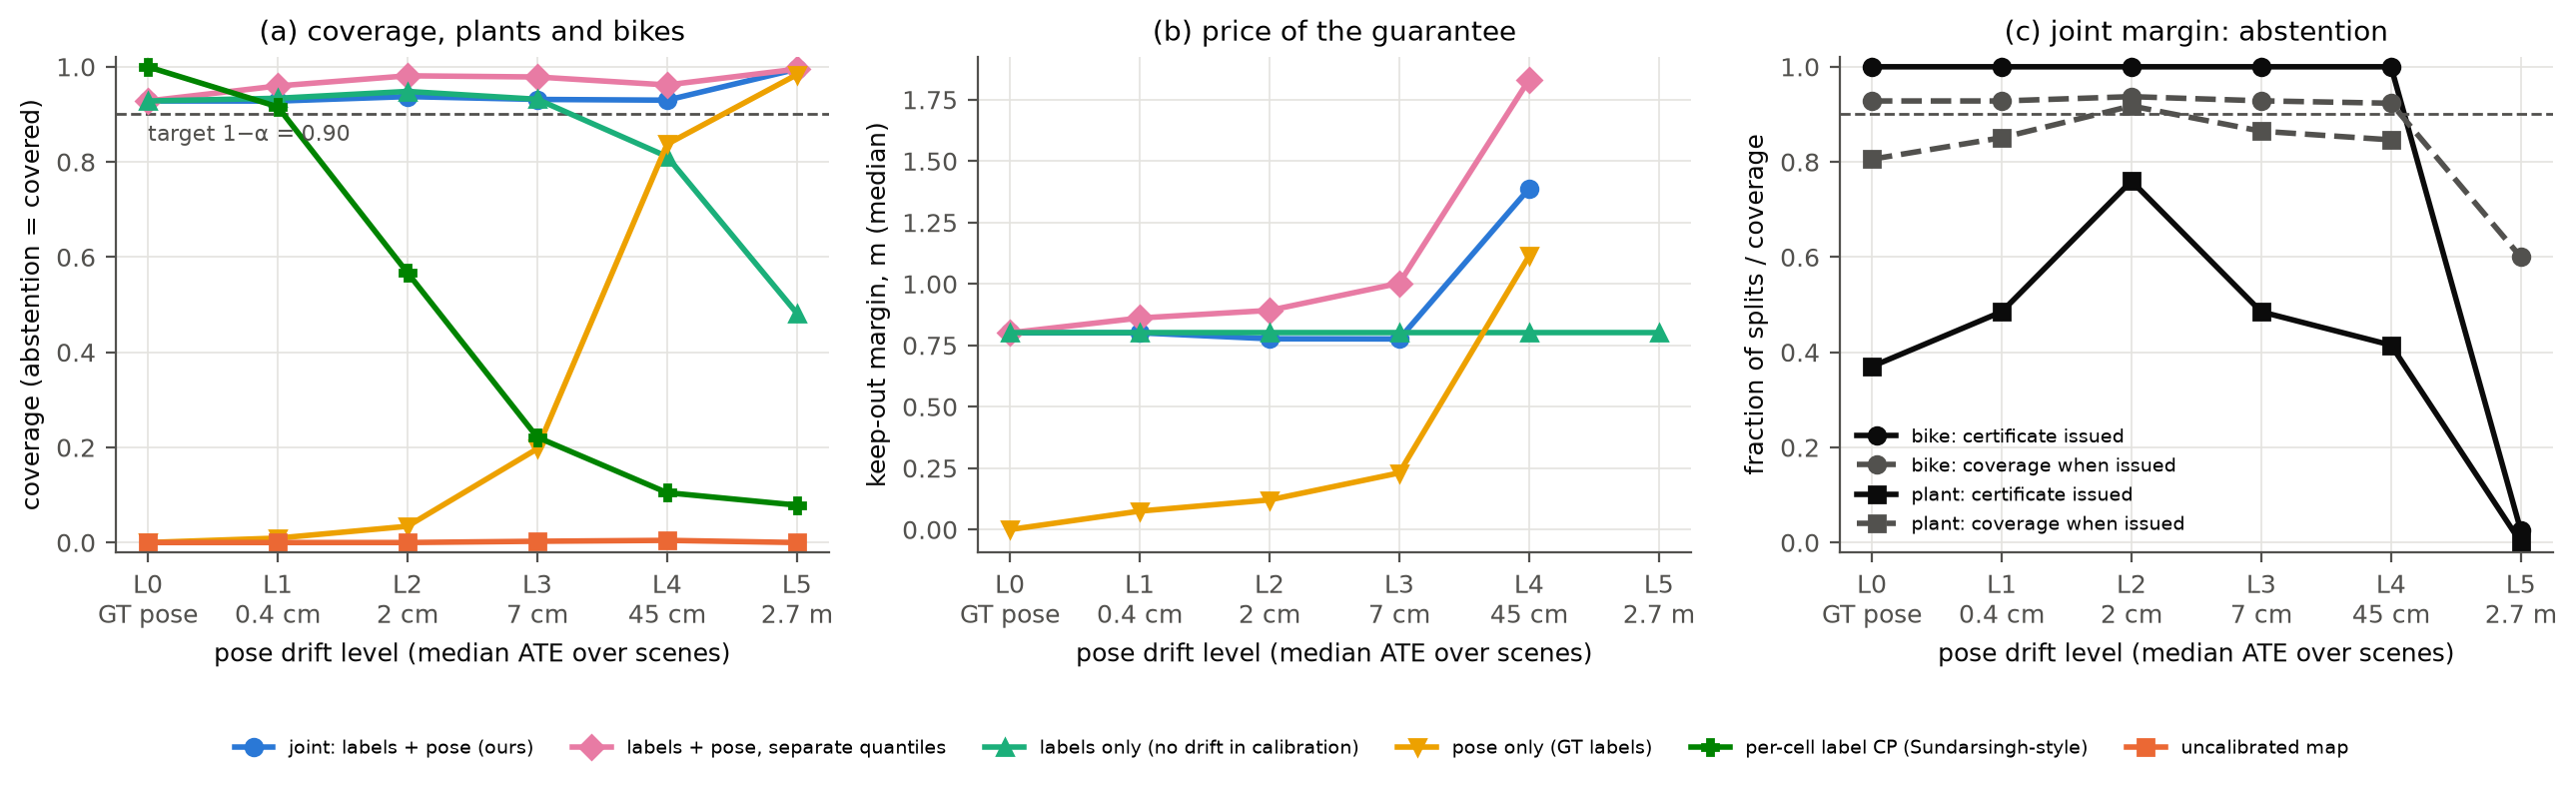
\includegraphics[width=\linewidth]{figures/coverage_headline.png}
\caption{Покрытие (слева) и запас (справа), среднее по растению и велосипеду}
\label{fig:coverage}
\end{figure}

Табл.~\ref{tab:coverage} и рис.~\ref{fig:coverage} проверяют гипотезы H1--H3. Карта без калибровки почти никогда не накрывает истинный объект целиком: детектор обрезает края.

Калибровка меток клеток даёт покрытие 1,00 без дрейфа, но лишь потому, что её порог $\lambda^\ast = 0$ объявляет возможным растением любую занятую клетку. Запаса в метрах у неё нет, поэтому сдвиг на 2~см уже снижает покрытие велосипеда до 0,73.

Запас «только метки» держится, пока дрейф мал по сравнению с ошибкой меток (до 7~см), и падает до 0,76 при 45~см (H1). Запас «только поза» не видит ошибок детектора: при дрейфе до 7~см его покрытие не выше 0,22 (H2).

Совместный запас держит 0,93--0,94 на всех уровнях. При 45~см он равен 1,18~м для велосипеда против 1,61~м у суммы отдельных запасов и 1,53 против 2,11~м для растения, то есть на 27--28\,\% меньше (H3).

Растение отказывается примерно в 60\,\% разбиений: в одной сцене детектор пропускает его целиком, а при 13 сценах запас равен максимуму. Тумба под ТВ отказывается в 71--95\,\% разбиений: в двух сценах из 21 детектор уверенно принимает её за скамейку или ковёр (промах 5,6 и 6,5~м). Для этого детектора гарантировать тумбу на уровне 90\,\% нельзя, и калибровка сообщает об этом.

\subsection{Миссии}\label{sec:missions}

\begin{figure}[H]
\centering
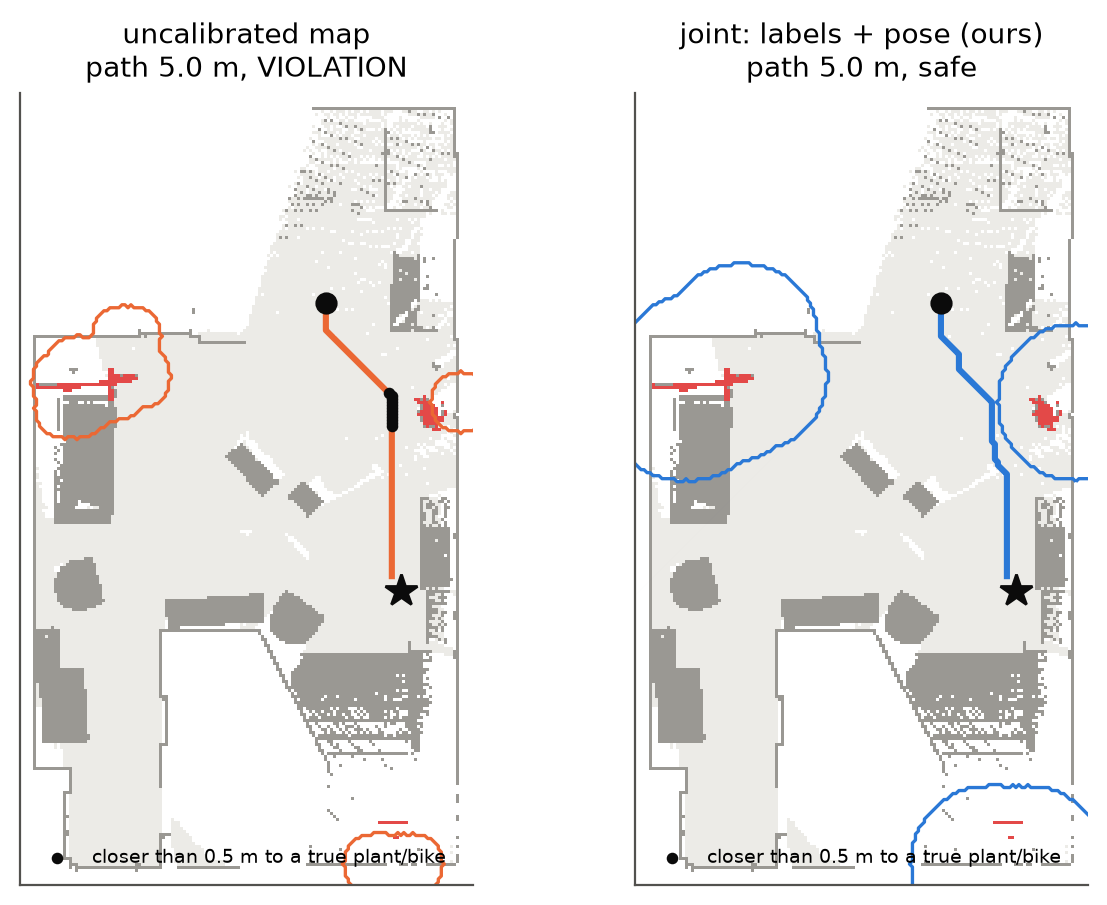
\includegraphics[width=0.7\linewidth]{figures/example_v3_sc0_staging_20_paper.png}
\caption{Трудная задача при дрейфе L2. Красное --- истинные растение и велосипед, серое --- препятствия, линия --- граница запретной зоны. Без калибровки зона не накрывает часть растения, и путь проходит ближе 0,5~м (чёрные точки); совместный запас накрывает объект}
\label{fig:example}
\end{figure}

\begin{table}[H]
\centering\small
\caption{Трудные задачи (растение и велосипед, 233 задачи): доля задач с найденным путём, доля опасных среди найденных путей, доля успешных миссий}
\label{tab:missions}
\begin{tabular}{lccccccccc}
\toprule
Ветка & \multicolumn{3}{c}{L0} & \multicolumn{3}{c}{L2} & \multicolumn{3}{c}{L4} \\
 & путь & наруш. & успех & путь & наруш. & успех & путь & наруш. & успех \\
\midrule
без калибровки & 0{,}99 & 0{,}27 & 0{,}73 & 0{,}97 & 0{,}32 & 0{,}65 & 0{,}26 & 0{,}34 & 0{,}17 \\
покадровая CP меток & 0{,}27 & 0{,}00 & 0{,}27 & 0{,}28 & 0{,}00 & 0{,}28 & 0{,}04 & 0{,}23 & 0{,}03 \\
только метки & 0{,}32 & 0{,}00 & 0{,}32 & 0{,}31 & 0{,}00 & 0{,}31 & 0{,}10 & 0{,}00 & 0{,}10 \\
только поза & 0{,}99 & 0{,}27 & 0{,}73 & 0{,}96 & 0{,}20 & 0{,}77 & 0{,}09 & 0{,}00 & 0{,}09 \\
раздельно (сумма) & 0{,}32 & 0{,}00 & 0{,}32 & 0{,}31 & 0{,}00 & 0{,}31 & 0{,}00 & 0{,}00 & 0{,}00 \\
\textbf{совместно} & 0{,}32 & 0{,}00 & 0{,}32 & 0{,}31 & 0{,}00 & 0{,}31 & 0{,}03 & 0{,}00 & 0{,}03 \\
оракул & 1{,}00 & 0{,}00 & 1{,}00 & 0{,}98 & 0{,}00 & 0{,}98 & 0{,}98 & 0{,}00 & 0{,}98 \\
\bottomrule
\end{tabular}

\end{table}

На трудных задачах планировщик без калибровки находит путь почти всегда, но 27--37\,\% его путей опасны (L0--L3). У всех вариантов с откалиброванным запасом опасных путей нет. Цена --- путь находится лишь в 30--32\,\% трудных задач, тогда как на истинной карте --- в 98--100\,\%. На случайных задачах совместный запас даёт 78\,\% успешных миссий без дрейфа и 68\,\% при дрейфе L3, без опасных путей. Без калибровки успешны 95 и 82\,\%, но 4--6\,\% миссий опасны.

Если запретными считаются все три класса, отказ тумбы переводит планировщик на запасной вариант, и путь находится лишь в 23\,\% трудных задач без дрейфа и в 5--8\,\% при дрейфе L2--L3.

\subsection{Сравнение с калибровкой меток в её условиях}\label{sec:comparison}

Успех миссий у~\cite{sundarsingh} (98,36\,\%) получен в другой постановке: открытые площадки, известная поза, пять классов, случайные задачи и режим исследования, когда пути нет. Поэтому мы сравниваем методы на наших сценах в их условиях. Поза известна. Словарь закрыт пятью классами: из 98 текстовых эмбеддингов детектора оставлены пять, что совпадает с перенастройкой словаря. Цель $1 - \alpha = 0{,}95$, задачи случайные. Режим исследования не воспроизводился.

\begin{table}[H]
\centering\scriptsize\setlength{\tabcolsep}{3.5pt}
\caption{Случайные задачи: покрытие (минимум по растению и велосипеду), доля успешных миссий и доля опасных миссий}
\label{tab:comparison}
\begin{tabular}{ll|ccc|ccc|cc|c}
\toprule
Условия & Дрейф & \multicolumn{3}{c|}{метки клеток} & \multicolumn{3}{c|}{\textbf{совместно}} & \multicolumn{2}{c|}{без калибровки} & оракул \\
 & & покр. & успех & опасно & покр. & успех & опасно & успех & опасно & успех \\
\midrule
закрытый словарь, 95\,\% & известна & 1{,}00 & 0{,}43 & 0{,}000 & 0{,}94 & 0{,}42 & 0{,}000 & 0{,}96 & 0{,}040 & 1{,}00 \\
 & L2 & 0{,}42 & 0{,}40 & 0{,}000 & 0{,}94 & 0{,}61 & 0{,}000 & 0{,}92 & 0{,}042 & 0{,}97 \\
 & L3 & 0{,}10 & 0{,}32 & 0{,}002 & 0{,}94 & 0{,}50 & 0{,}000 & 0{,}82 & 0{,}049 & 0{,}97 \\
\midrule
открытый словарь, 90\,\% & известна & 1{,}00 & 0{,}43 & 0{,}000 & 0{,}93 & 0{,}78 & 0{,}000 & 0{,}95 & 0{,}043 & 1{,}00 \\
 & L2 & 0{,}41 & 0{,}40 & 0{,}000 & 0{,}93 & 0{,}74 & 0{,}000 & 0{,}91 & 0{,}050 & 0{,}97 \\
 & L3 & 0{,}10 & 0{,}32 & 0{,}002 & 0{,}94 & 0{,}68 & 0{,}000 & 0{,}82 & 0{,}056 & 0{,}97 \\
 & L4 & 0{,}03 & 0{,}09 & 0{,}000 & 0{,}93 & 0{,}17 & 0{,}000 & 0{,}29 & 0{,}021 & 0{,}98 \\
\bottomrule
\end{tabular}

\end{table}

\begin{figure}[H]
\centering
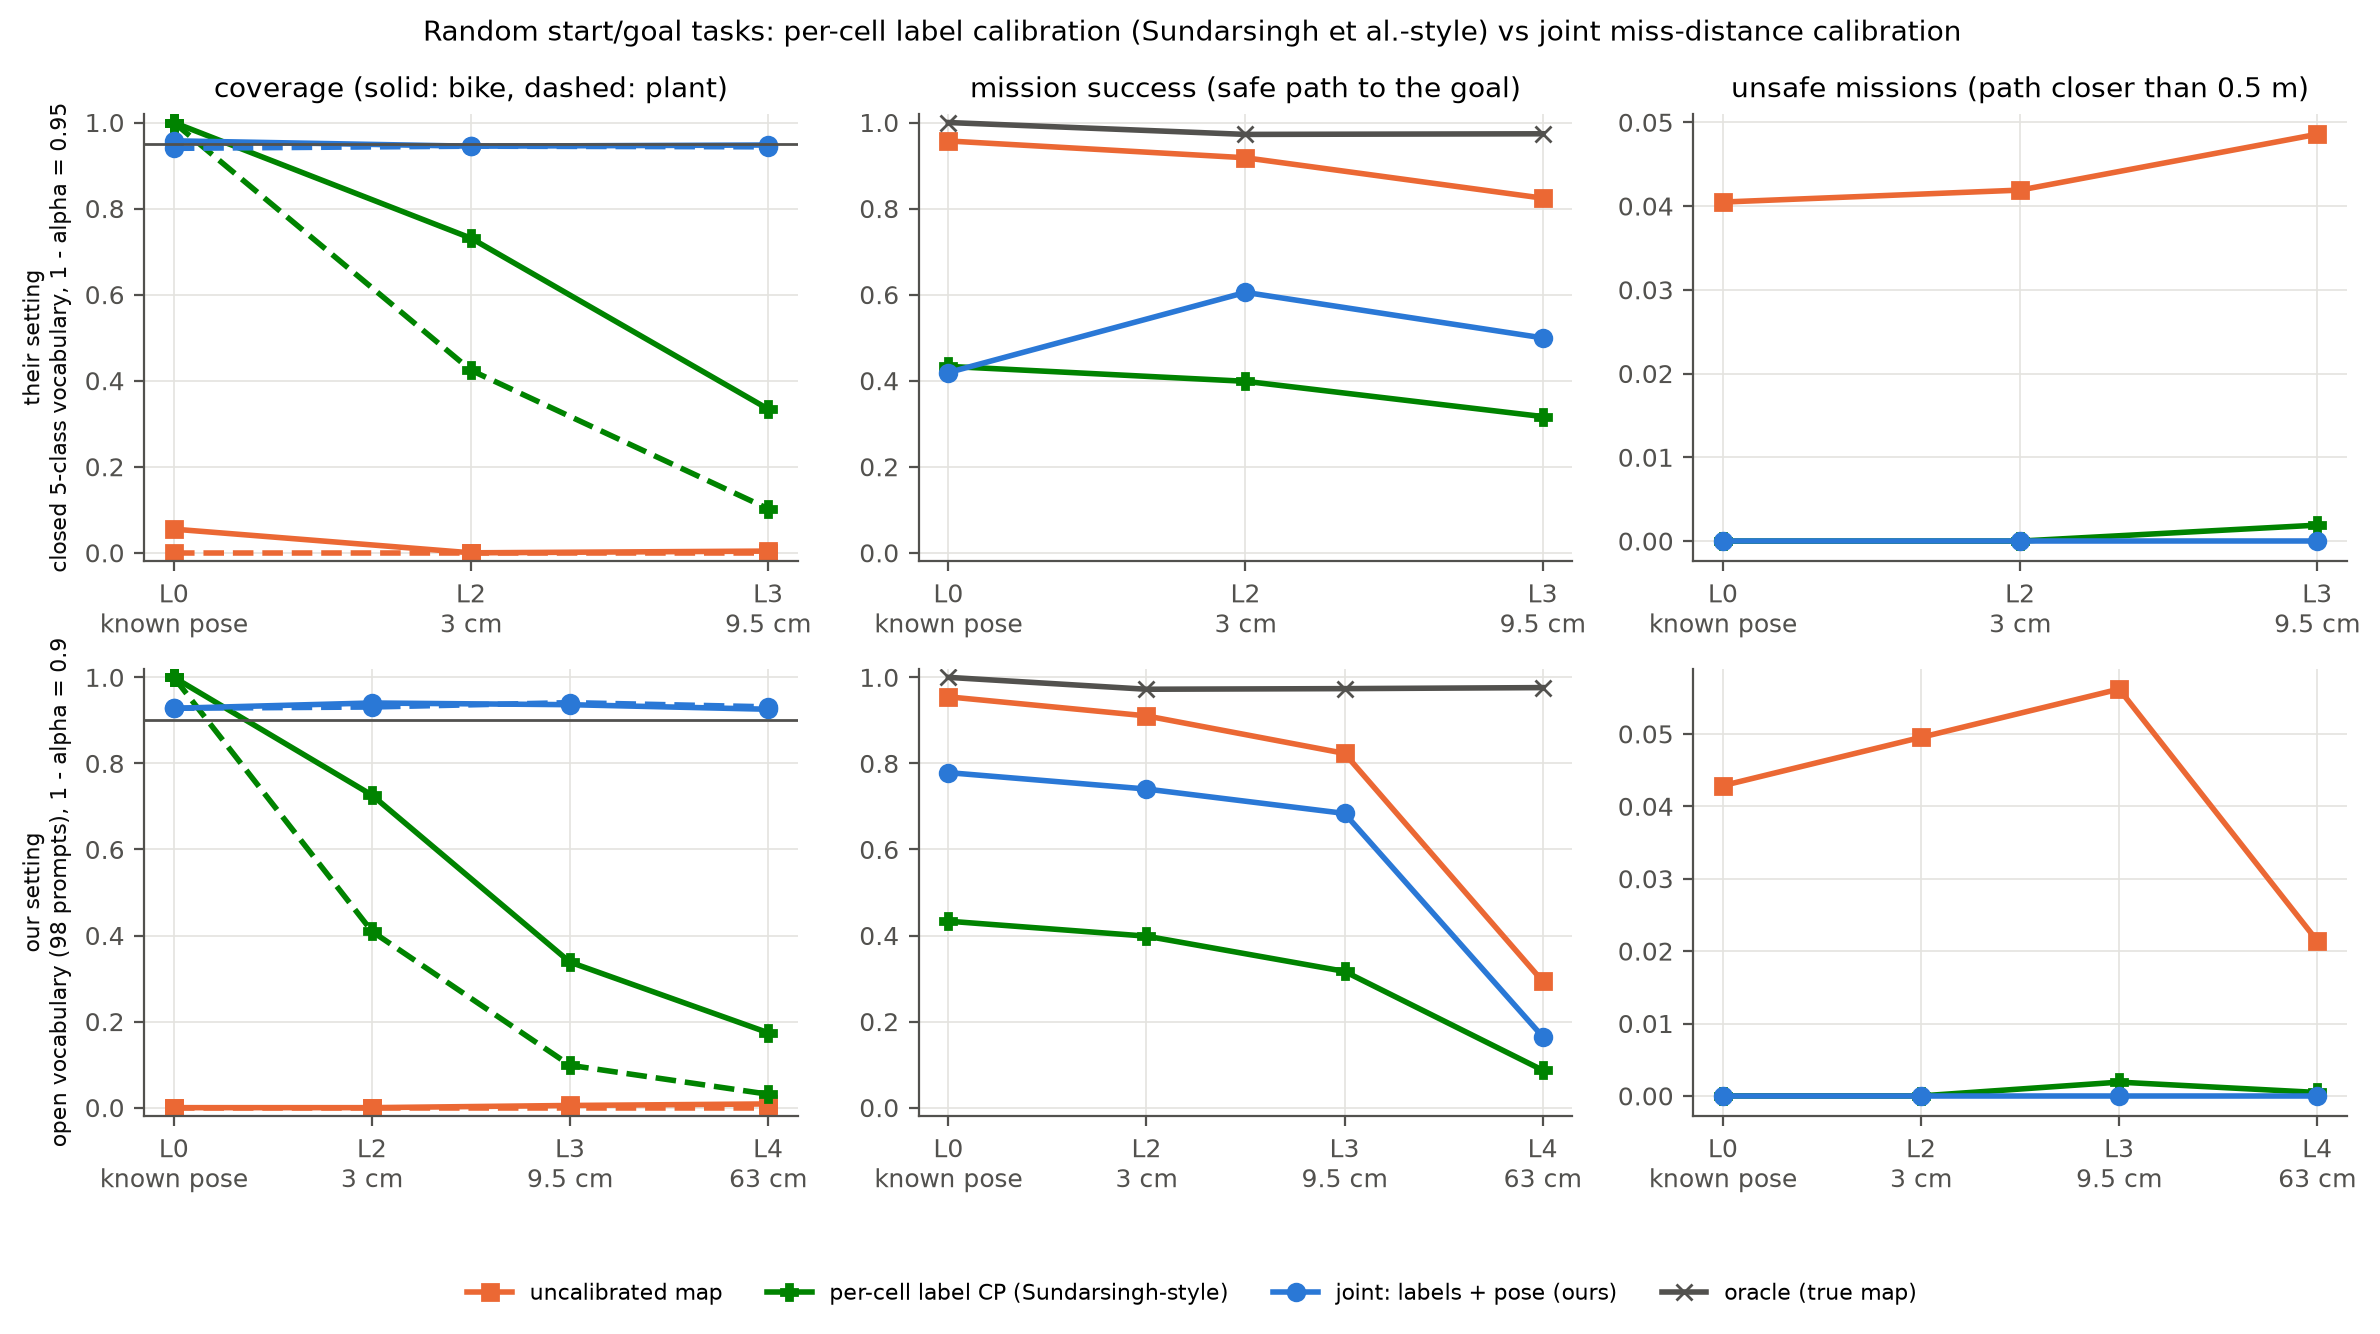
\includegraphics[width=\linewidth]{figures/comparison.png}
\caption{Калибровка меток клеток~\cite{sundarsingh} и совместный запас на случайных задачах. Сверху --- закрытый словарь и $1 - \alpha = 0{,}95$, снизу --- открытый словарь и $1 - \alpha = 0{,}9$}
\label{fig:comparison}
\end{figure}

В их условиях методы равны: 0,43 и 0,42 успешных миссий, опасных нет (табл.~\ref{tab:comparison}). При дрейфе 2 и 7~см покрытие калибровки меток падает до 0,42 и 0,10, совместный запас держит 0,94 и даёт больше успешных миссий: 0,61 и 0,50 против 0,40 и 0,32. С открытым словарём совместный запас даёт в 1,8 раза больше успешных миссий уже при известной позе.

Калибровка меток у нас вырождается: порог $\lambda^\ast = 0$ в обоих словарях. Мы проверили, не виновата ли мелкая сетка, и повторили обе калибровки на сетках 5, 25, 50 и 100~см. Порог равен нулю на всех; запретная зона калибровки меток занимает 64\,\% свободного пространства при 5~см и всё пространство при 1~м. Причина в полных промахах детектора: если в одной калибровочной сцене до части объекта не дошло ни одного наблюдения его класса, худшая клетка даёт счёт 1 и порог 0. Множество меток может сказать только «эта клетка может быть растением». Расстояние говорит «растение где-то рядом», и это остаётся полезным, когда детектор теряет части объектов.

\subsection{Цена гарантии}\label{sec:price}

\begin{table}[H]
\centering\small
\caption{Уровень риска $\alpha$ при дрейфе L3: покрытие и запас совместного варианта, доля отказов для растения, доля трудных задач с найденным путём и доля опасных миссий. При $\alpha = 0{,}05$ разбиение 19/2}
\label{tab:alpha}
\begin{tabular}{c|cc|cc|c|cc|cc}
\toprule
$\alpha$ & \multicolumn{2}{c|}{покрытие} & \multicolumn{2}{c|}{$\hat r$, м} & отказ & \multicolumn{2}{c|}{трудные: путь} & \multicolumn{2}{c}{случайные: успех} \\
 & раст. & велос. & раст. & велос. & раст. & совм. & оракул & совм. & оракул \\
\midrule
0{,}05 & 0{,}95 & 0{,}95 & 0{,}85 & 0{,}76 & 0{,}70 & 0{,}10 & 0{,}99 & 0{,}34 & 0{,}97 \\
0{,}10 & 0{,}93 & 0{,}93 & 0{,}80 & 0{,}75 & 0{,}52 & 0{,}30 & 0{,}99 & 0{,}68 & 0{,}97 \\
0{,}20 & 0{,}86 & 0{,}86 & 0{,}74 & 0{,}70 & 0{,}00 & 0{,}31 & 0{,}99 & --- & --- \\
0{,}30 & 0{,}72 & 0{,}72 & 0{,}60 & 0{,}50 & 0{,}00 & 0{,}31 & 0{,}99 & 0{,}71 & 0{,}97 \\
\bottomrule
\end{tabular}

\end{table}

Повышение риска почти не добавляет решаемых задач (табл.~\ref{tab:alpha}). С $\alpha = 0{,}1$ до 0,3 запас уменьшается на 0,2--0,25~м, а доля трудных задач с путём растёт с 30 до 31\,\%; покрытие при этом следует за $1 - \alpha$.

Лучшие маски тоже не уменьшают запас. MobileSAM~\cite{mobilesam}, получающий на вход рамки детектора, снижает медианный промах велосипеда с 0,43 до 0,05~м. Однако наихудшая сцена сохраняет промах 0,75~м, и при 13 калибровочных сценах запас равен именно ей. С масками SAM карта без калибровки безопасна при известной позе (опасных путей нет), но не при дрейфе (9,5\,\% опасных путей при L3).

Запас определяет хвост ошибок восприятия. Уменьшить его можно, убрав наихудшие ошибки детектора или взяв больше калибровочных сцен.

\subsection{Когда сумма запасов недопокрывает}\label{sec:composition}

На синтетическом дрейфе сумма отдельных запасов только переплачивает: дрейф независим от ошибок детектора. Чтобы проверить утверждение~\ref{prop:sep}, мы оставили реальные ошибки меток и заменили дрейф сценовой смесью. В $k$ сценах из 21 происходит сбой локализации (реализации уровня L5), в остальных дрейф пренебрежимо мал (L1). Сцены со сбоем выбираются там, где метки хуже всего, где они лучше всего, или случайно. Уровень $\alpha = 0{,}3$ выбран потому, что при $\alpha = 0{,}1$ и 13 сценах любой сбой попадает в максимум.

\begin{figure}[H]
\centering
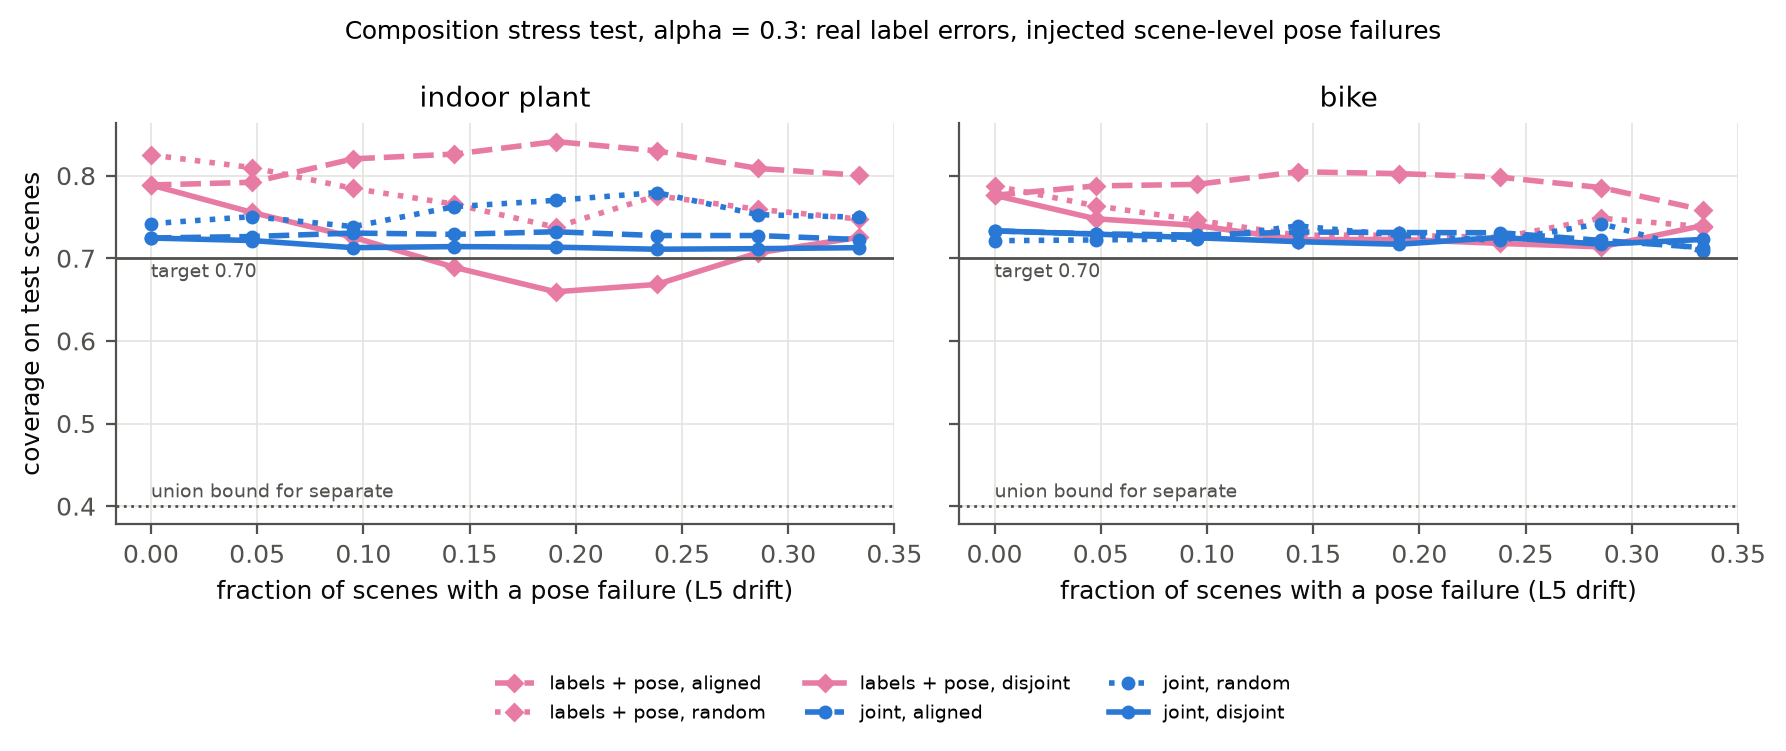
\includegraphics[width=\linewidth]{figures/composition_stress_a03_L5.png}
\caption{Покрытие суммы отдельных запасов (розовое) и совместного запаса (синее) в зависимости от доли сцен со сбоем локализации; $1 - \alpha = 0{,}7$, нижняя линия --- граница $1 - 2\alpha$}
\label{fig:composition}
\end{figure}

Если сбои совпадают с плохими метками, сумма даёт 0,76--0,84. Если сбои приходятся на сцены с хорошими метками, она опускается до 0,66 при цели 0,70 (растение, 19--24\,\% сцен со сбоем). Совместный запас даёт 0,71--0,78 при любом расположении сбоев (рис.~\ref{fig:composition}).

\subsection{Реальная одометрия и другие сцены}\label{sec:variants}

\begin{table}[H]
\centering\scriptsize\setlength{\tabcolsep}{3.5pt}
\caption{Проверка упрощений: покрытие и медианный запас (м), $\alpha = 0{,}1$; $^\dagger$ --- вариант отказывается в половине разбиений или чаще, приведён запас в остальных}
\label{tab:variants}
\begin{tabular}{l|cccccc|cccccc}
\toprule
Вариант & \multicolumn{6}{c|}{велосипед} & \multicolumn{6}{c}{растение} \\
 & \multicolumn{2}{c}{метки} & \multicolumn{2}{c}{раздельно} & \multicolumn{2}{c}{\textbf{совместно}} & \multicolumn{2}{c}{метки} & \multicolumn{2}{c}{раздельно} & \multicolumn{2}{c}{\textbf{совместно}} \\
 & покр. & $\hat q$ & покр. & $\hat q$ & покр. & $\hat q$ & покр. & $\hat q$ & покр. & $\hat q$ & покр. & $\hat q$ \\
\midrule
рамка + глубина, L0 & 0{,}93 & 0{,}75 & 0{,}93 & 0{,}75 & 0{,}93 & 0{,}75 & 0{,}93 & 0{,}85$^\dagger$ & 0{,}93 & 0{,}85$^\dagger$ & 0{,}93 & 0{,}85$^\dagger$ \\
рамка + глубина, L3 & 0{,}93 & 0{,}75 & 0{,}99 & 0{,}90 & 0{,}94 & 0{,}75 & 0{,}94 & 0{,}85$^\dagger$ & 0{,}96 & 1{,}09$^\dagger$ & 0{,}94 & 0{,}81$^\dagger$ \\
рамка + глубина, L4 & 0{,}76 & 0{,}75 & 0{,}97 & 1{,}61 & 0{,}93 & 1{,}18 & 0{,}86 & 0{,}85$^\dagger$ & 0{,}95 & 2{,}11$^\dagger$ & 0{,}93 & 1{,}53$^\dagger$ \\
MobileSAM, L0 & 0{,}93 & 0{,}75 & 0{,}93 & 0{,}75 & 0{,}93 & 0{,}75 & 0{,}93 & 0{,}61$^\dagger$ & 0{,}93 & 0{,}61$^\dagger$ & 0{,}93 & 0{,}61$^\dagger$ \\
MobileSAM, L3 & 0{,}93 & 0{,}75 & 0{,}97 & 0{,}90 & 0{,}93 & 0{,}75 & 0{,}94 & 0{,}61$^\dagger$ & 0{,}95 & 0{,}86$^\dagger$ & 0{,}95 & 0{,}61$^\dagger$ \\
MobileSAM, L4 & 0{,}78 & 0{,}75 & 0{,}98 & 1{,}61 & 0{,}93 & 1{,}03 & 0{,}82 & 0{,}61$^\dagger$ & 0{,}94 & 1{,}92$^\dagger$ & 0{,}95 & 1{,}63$^\dagger$ \\
ВО, каждый 2-й кадр & 0{,}67 & 0{,}75 & 0{,}92 & 2{,}46$^\dagger$ & 0{,}93 & 1{,}95$^\dagger$ & 0{,}74 & 0{,}85$^\dagger$ & 0{,}97 & 2{,}98$^\dagger$ & 0{,}96 & 2{,}31$^\dagger$ \\
ВО, каждый 4-й кадр & 0{,}51 & 0{,}75 & 0{,}97 & 3{,}15$^\dagger$ & 0{,}96 & 2{,}41$^\dagger$ & 0{,}75 & 0{,}85$^\dagger$ & 0{,}99 & 3{,}46$^\dagger$ & 0{,}97 & 2{,}42$^\dagger$ \\
HM3D (OOD), L0 & --- & --- & --- & --- & --- & --- & 0{,}50 & 0{,}85 & 0{,}50 & 0{,}85 & 0{,}50 & 0{,}85 \\
HM3D (OOD), L3 & --- & --- & --- & --- & --- & --- & 0{,}50 & 0{,}85 & 0{,}50 & 1{,}07 & 0{,}50 & 0{,}82 \\
\bottomrule
\end{tabular}

\end{table}

Одометрия кадр к кадру без замыканий циклов ошибается неравномерно: ATE по сценам от 3,5~см до 3,9~м, медиана 78~см. Ошибка набирается в основном на отдельных шагах --- поворотах на месте у стен. Запас «только метки» молча теряет покрытие: 0,67 для велосипеда и 0,74 для растения (табл.~\ref{tab:variants}). Совместный запас остаётся валидным (0,93 и 0,96), но отказывается в 60 и 86\,\% разбиений. В миссиях планировщик без калибровки находит путь в 23\,\% задач, и 44\,\% этих путей опасны; совместный вариант отказывается в 89\,\% задач. При такой ошибке позы полезной гарантии нет, и метод сообщает об этом вместо ложного сертификата.

Запасы, откалиброванные на ReplicaCAD, мы проверили на сценах HM3D~\cite{hm3d} из OSMa-Bench --- реальных сканах домов в условии \texttt{no\_lights}. Растение видно с траектории лишь в двух из шести одноэтажных сцен. В одной детектор находит его (промах 0,18~м), в другой делит декоративное растение между классами «подставка», «скульптура» и «горшок» (промах 2,9~м). Покрытие 0,5 на двух сценах --- иллюстрация, а не оценка: гарантия не переносится на другое семейство сцен, калибровать нужно там, где работает робот.

\subsection{Качество карты и безопасность}\label{sec:h4}

Для каждой сцены мы сопоставили mIoU карты при точных позах с долей опасных путей планировщика без калибровки. Ранговая корреляция $\rho = -0{,}16$ ($p = 0{,}57$, 15 сцен); для IoU одних запретных классов знак даже обратный ($\rho = +0{,}51$, $p = 0{,}05$). mIoU усредняет по клеткам, а безопасность определяет наихудший объект в сцене (H4).

\section{Обсуждение}\label{sec:discussion}

\textbf{Что подтвердилось и что нет.} Запас, откалиброванный по одной ошибке, перестаёт работать, когда действует вторая (H1, H2), а совместный запас не больше суммы двух отдельных и при большом дрейфе меньше её на четверть (H3). Связи mIoU с безопасностью на 15 сценах не видно, но и отсутствие её не доказано (H4). Три ожидания не оправдались. Положительная корреляция ошибок делает сумму запасов консервативнее, а недопокрытие возникает, когда редкие сбои локализации и ошибки меток приходятся на разные сцены, и оно невелико. Множества меток выродились не из-за полных пропусков, а из-за обрезанных краёв. Реальная одометрия ошибается не плавно, как модель дрейфа, а скачками.

\textbf{Отрицательные результаты} (получены на предыдущей версии конвейера и не пересчитывались). Выпуклая оболочка и морфологическое замыкание областей не меняют промах: пропущенная часть объекта лежит вне найденного фрагмента, а не в дырах внутри него. Запас, зависящий от уверенности фрагмента, не уменьшил запретную зону.

\textbf{Главное узкое место} --- уверенный пропуск или подмена класса целого объекта. Пока калибровочных сцен не меньше $1/\alpha - 1$, но меньше $2/\alpha - 1$, запас равен наихудшему промаху, и одна такая сцена заставляет класс отказываться в значительной доле разбиений; при 19 сценах растение почти не отказывается. Более сильные детекторы убирают пропуск растения, но у каждого из трёх проверенных находится свой целиком пропущенный класс; подмену тумбы создаёт словарь, а закрытый словарь превращает её в ложные срабатывания. Объединение детекторов по максимуму это узкое место снимает, а проверка находок и голосование возвращают его: гарантия чувствительна к полноте, а не к точности. Метрики качества карты этого не отражают, и в протокол бенчмарков вроде OSMa-Bench естественно добавить долю сцен, где объект пропущен или подменён целиком.

\textbf{Какую гарантию требовать.} Гарантия «каждый объект внутри запаса» дорога, потому что за неё платят и объекты, мимо которых не идёт ни один путь. Гарантия на ожидаемую долю опасных миссий (разд.~\ref{sec:crc}) почти не уменьшает число решённых задач, но допускает целиком опасную сцену. Для реальной локализации важен хвост ошибок: SLAM с замыканиями втрое снижает медианную ошибку, но запас задают сцены без замыканий.

\textbf{Ограничения.}
\begin{itemize}[nosep]
  \item Одно семейство из 21 симулированной сцены (пять групп расстановок мебели) и одно условие освещения; бутстреп по сценам эту кластеризацию не учитывает. Покрытие на случайных разбиениях одних и тех же сцен выполняется по построению; о поведении на новых сценах говорят лишь бутстреп-интервалы шириной 0,1--0,15, проверка с отложенной планировкой и две сцены HM3D.
  \item Основной дрейф синтетический и не зависит от ошибок детектора. Реальная локализация проверена одометрией и собственным SLAM с замыканиями на основе Open3D; промышленные системы (ORB-SLAM3, RTAB-Map) не проверялись.
  \item Восприятие --- детектор рамок с масками по глубине или MobileSAM, а не полный картограф.
  \item Гарантия маргинальна по калибровочным выборкам и поклассова; для нескольких классов сразу она слабее, $1 - |\mathcal K_m|\,\alpha$.
  \item Основная гарантия относится к плану в момент запроса (допущение~\ref{as:exec}). Исполнение с дрейфом проверено моделью дрейфа, а не реальным роботом; запас на исполнение калибруется по объединённой выборке путей, и его обменяемость приближённая. Столкновения с препятствиями не покрываются. Дискретизация может съесть до 7~см безопасного расстояния.
  \item Семейство трудных задач и пара запретных классов для миссий выбраны после первых прогонов; множества меток реализованы нами на итоговой карте, без режима исследования авторов.
\end{itemize}

\section{Заключение}

Расстояние промаха в системе координат планировщика --- одна калибруемая величина, которая даёт планировщику гарантию сразу против ошибки метки и ошибки позы и честно отказывается, когда гарантия была бы бесполезной. Запасы по одной ошибке теряют покрытие под действием другой, сумма отдельных запасов переплачивает или недопокрывает в зависимости от неизвестного расположения сбоев, а калибровка множеств меток вырождается в запрет всего занятого. Цену гарантии задаёт наихудшая ошибка восприятия или локализации среди калибровочных сцен. Её снижают объединение детекторов (полнота важнее точности) и переход к гарантии на долю опасных миссий; исполнение с дрейфом до 7~см не ломает её относительно запретных классов, хотя 1--9\,\% исполнений задевают препятствия. Следующие шаги --- больше калибровочных сцен (например, данные OSMa-Bench++), SLAM, находящий замыкания во всех сценах, перелокализация во время движения и полный открытословарный картограф вместо детектора рамок.

\begin{thebibliography}{99}
\footnotesize

\bibitem{conceptgraphs} ConceptGraphs: Open-Vocabulary 3D Scene Graphs for Perception and Planning / Q.~Gu [и~др.] // 2024 IEEE International Conference on Robotics and Automation (ICRA). --- 2024. --- P.~5021--5028. --- DOI 10.1109/ICRA57147.2024.10610243.

\bibitem{osmabench} OSMa-Bench: Evaluating Open Semantic Mapping Under Varying Lighting Conditions / M.~Popov [и~др.] // 2025 IEEE/RSJ International Conference on Intelligent Robots and Systems (IROS). --- 2025. --- P.~10786--10791. --- DOI 10.1109/IROS60139.2025.11247603.

\bibitem{survey3dsg} 3D Scene Graphs: Open Challenges and Future Directions / D.~Rotondi [и~др.] // arXiv preprint. --- 2026. --- arXiv:2606.19383. --- (Приглашённая статья для Annual Review of Control, Robotics, and Autonomous Systems, т.~10, по комментарию arXiv.)

\bibitem{gentle} Angelopoulos~A.~N. A Gentle Introduction to Conformal Prediction and Distribution-Free Uncertainty Quantification / A.~N.~Angelopoulos, S.~Bates // arXiv preprint. --- 2021. --- arXiv:2107.07511.

\bibitem{sundarsingh} Safe Planning in Unknown Environments Using Conformalized Semantic Maps / D.~S.~Sundarsingh [и~др.] // IEEE Robotics and Automation Letters. --- 2026. --- Vol.~11, no.~4. --- P.~4921--4928. --- DOI 10.1109/LRA.2026.3668466.

\bibitem{pwc} Perceive With Confidence: Statistical Safety Assurances for Navigation with Learning-Based Perception / Z.~Mei [и~др.] // The International Journal of Robotics Research. --- 2025. --- Vol.~45, no.~6. --- P.~938--967. --- DOI 10.1177/02783649251378151.

\bibitem{baral} Baral~R. Marginal Calibration Does Not Compose: Hidden Dependence in Modular Robot Navigation / R.~Baral // arXiv preprint. --- 2026. --- arXiv:2609.23731. --- (Воркшоп «Rethinking Uncertainty for Modern Robotics Paradigms», IROS~2026.)

\bibitem{osmabenchpp} Kurkova~R. OSMa-Bench++: Toward Open-Ended Benchmarking of Semantic Mapping for Manipulation with Prompt-Generated Synthetic Scenes / R.~Kurkova, M.~Popov, S.~Kolyubin // arXiv preprint. --- 2026. --- arXiv:2605.26831. --- (Воркшоп ICRA~2026 «Open Challenges for Rigorous Robot Perception».)

\bibitem{overconf} Correia Marques~J.~M. On the Overconfidence Problem in Semantic 3D Mapping / J.~M.~Correia Marques, A.~Zhai, S.~Wang, K.~Hauser // 2024 IEEE International Conference on Robotics and Automation (ICRA). --- 2024. --- P.~11095--11102. --- DOI 10.1109/ICRA57147.2024.10611306.

\bibitem{tchuiev} Tchuiev~V. Epistemic uncertainty aware semantic localization and mapping for inference and belief space planning / V.~Tchuiev, V.~Indelman // Artificial Intelligence. --- 2023. --- Vol.~319. --- P.~103903. --- DOI 10.1016/j.artint.2023.103903.

\bibitem{lindemann} Safe Planning in Dynamic Environments using Conformal Prediction / L.~Lindemann [и~др.] // IEEE Robotics and Automation Letters. --- 2023. --- Vol.~8, no.~8. --- P.~5116--5123. --- DOI 10.1109/LRA.2023.3292071.

\bibitem{yang2023} Safe Perception-Based Control Under Stochastic Sensor Uncertainty Using Conformal Prediction / S.~Yang, G.~J.~Pappas, R.~Mangharam, L.~Lindemann // 2023 62nd IEEE Conference on Decision and Control (CDC). --- 2023. --- P.~6072--6078. --- DOI 10.1109/CDC49753.2023.10384075.

\bibitem{shin2026} Shin~J. From Prediction Uncertainty to Conformalized Distance Fields for Safe Motion Planning / J.~Shin, Y.~Ra, I.~Yang // arXiv preprint. --- 2026. --- arXiv:2607.00776.

\bibitem{score} Kim~E.~M. SCORE: Shape-Conforming Regions for Flight in Enclosed, Degraded Environments / E.~M.~Kim, J.-K.~Kim // arXiv preprint. --- 2026. --- arXiv:2608.15289.

\bibitem{learnablecp} Learnable Conformal Prediction with Context-Aware Nonconformity Functions for Robotic Planning and Perception / D.~Kumar [и~др.] // 2026 IEEE International Conference on Robotics and Automation (ICRA). --- 2026. --- arXiv:2509.21955. --- (Сверка версии в трудах ICRA с arXiv не проводилась.)

\bibitem{tightening} Natraj~S. Conformal Constraint Tightening for Chance-Constrained Motion Planning with Unknown Dynamics / S.~Natraj, B.~Sinopoli, Y.~Kantaros // arXiv preprint. --- 2026. --- arXiv:2607.22409.

\bibitem{calafiore2026} Calafiore~G.~C. Bridging Conformal Prediction and Scenario Optimization: Discarded Constraints and Modular Risk Allocation / G.~C.~Calafiore // arXiv preprint. --- 2026. --- arXiv:2603.19396.

\bibitem{mahajan} Mahajan~R. Finite-Sample Conformal Coverage Recovery via Fusion under Degraded Local Guarantees in Occupancy Map Estimation / R.~Mahajan, A.~Raghavan, K.~H.~Johansson // arXiv preprint. --- 2026. --- arXiv:2607.14906.

\bibitem{barber2023} Conformal prediction beyond exchangeability / R.~F.~Barber, E.~J.~Cand\`es, A.~Ramdas, R.~J.~Tibshirani // The Annals of Statistics. --- 2023. --- Vol.~51, no.~2. --- DOI 10.1214/23-AOS2276.

\bibitem{pposemem} P-POSEMEM: Projective Semantic Memory for Consistent Language Grounding under Pose-Graph Rewrites / H.~Sier [и~др.] // arXiv preprint. --- 2026. --- arXiv:2609.15475.

\bibitem{habitat2} Habitat 2.0: Training Home Assistants to Rearrange their Habitat / A.~Szot [и~др.] // Advances in Neural Information Processing Systems (NeurIPS). --- 2021. --- arXiv:2106.14405.

\bibitem{yoloworld} YOLO-World: Real-Time Open-Vocabulary Object Detection / T.~Cheng [и~др.] // 2024 IEEE/CVF Conference on Computer Vision and Pattern Recognition (CVPR). --- 2024. --- P.~16901--16911. --- DOI 10.1109/CVPR52733.2024.01599.

\bibitem{open3d} Zhou~Q.-Y. Open3D: A Modern Library for 3D Data Processing / Q.-Y.~Zhou, J.~Park, V.~Koltun // arXiv preprint. --- 2018. --- arXiv:1801.09847.

\bibitem{steinbrucker} Steinbr\"ucker~F. Real-time visual odometry from dense RGB-D images / F.~Steinbr\"ucker, J.~Sturm, D.~Cremers // 2011 IEEE International Conference on Computer Vision Workshops (ICCV Workshops). --- 2011. --- P.~719--722. --- DOI 10.1109/ICCVW.2011.6130321.

\bibitem{mobilesam} Faster Segment Anything: Towards Lightweight SAM for Mobile Applications / C.~Zhang, D.~Han, Y.~Qiao [и~др.] // arXiv preprint. --- 2023. --- arXiv:2306.14289.

\bibitem{hm3d} Habitat-Matterport 3D Dataset (HM3D): 1000 Large-scale 3D Environments for Embodied AI / S.~K.~Ramakrishnan, A.~Gokaslan, E.~Wijmans [и~др.] // NeurIPS Datasets and Benchmarks. --- 2021. --- arXiv:2109.08238.

\end{thebibliography}

\end{document}
